\documentclass[UTF8]{ctexart}

\newcommand\subtitle[1]{{\small #1}}

\title{\textbf{2024-2025学年第2学期}\\ \textbf{C++课程作业}\\ \subtitle{仿QQ的聊天程序} \\ \small 班级:24-1} % 在这里直接添加班级信息
\author{\textbf{成员:}\\ \underline{2410120025 郭警豪} \\ \underline{2410120034 陈晓豪}
}
\date{\today}

\usepackage{graphicx}
\begin{document}
\maketitle
\tableofcontents
\newpage
\section{程序说明}


\textbf{我们小组开发了一个仿QQ的聊天程序,主要实现了以下功能:}


\begin{itemize}
	\item 用户注册与登录:用户可以通过输入用户名和密码进行注册和登录。
	\item 好友管理:用户可以搜索其他用户并添加为好友,查看好友列表,同意或拒绝好友申请。
	\item 聊天功能:用户可以与好友进行单聊,发送和接收文本消息,并查看历史聊天记录。
\end{itemize}

\textbf{该程序使用Qt框架开发客户端界面,Sqlite数据库存储用户信息和聊天记录,通过Socket实现客户端与服务端的通信。}

\section{程序分析}
\subsection{功能需求}
\begin{itemize}
	\item 用户管理**:支持用户注册、登录,存储用户信息。
	\item 好友管理**:支持搜索用户、添加好友、查看好友列表、处理好友申请。
	\item 聊天功能**:支持单聊,发送和接收消息,查看历史消息。
\end{itemize}	
\subsection{性能需求}
\begin{itemize}
	\item 响应速度:用户操作(如登录、发送消息)应在短时间内得到响应。
	\item 数据存储:用户信息和聊天记录需安全存储,支持历史消息查询。
	\item 并发处理:支持多个用户同时在线,处理并发通信。
\end{itemize}
	
\section{程序设计}
\subsection{设计思路}
\begin{itemize}
	\item 客户端:使用Qt框架开发图形用户界面,实现用户交互功能。
	\item 服务端:处理客户端请求,与数据库交互,存储和查询数据。
	\item 通信:通过Socket实现客户端与服务端的通信,传输JSON格式的数据。
\end{itemize}
\subsection{数据库设计}
\begin{figure}[h]
	\centering
	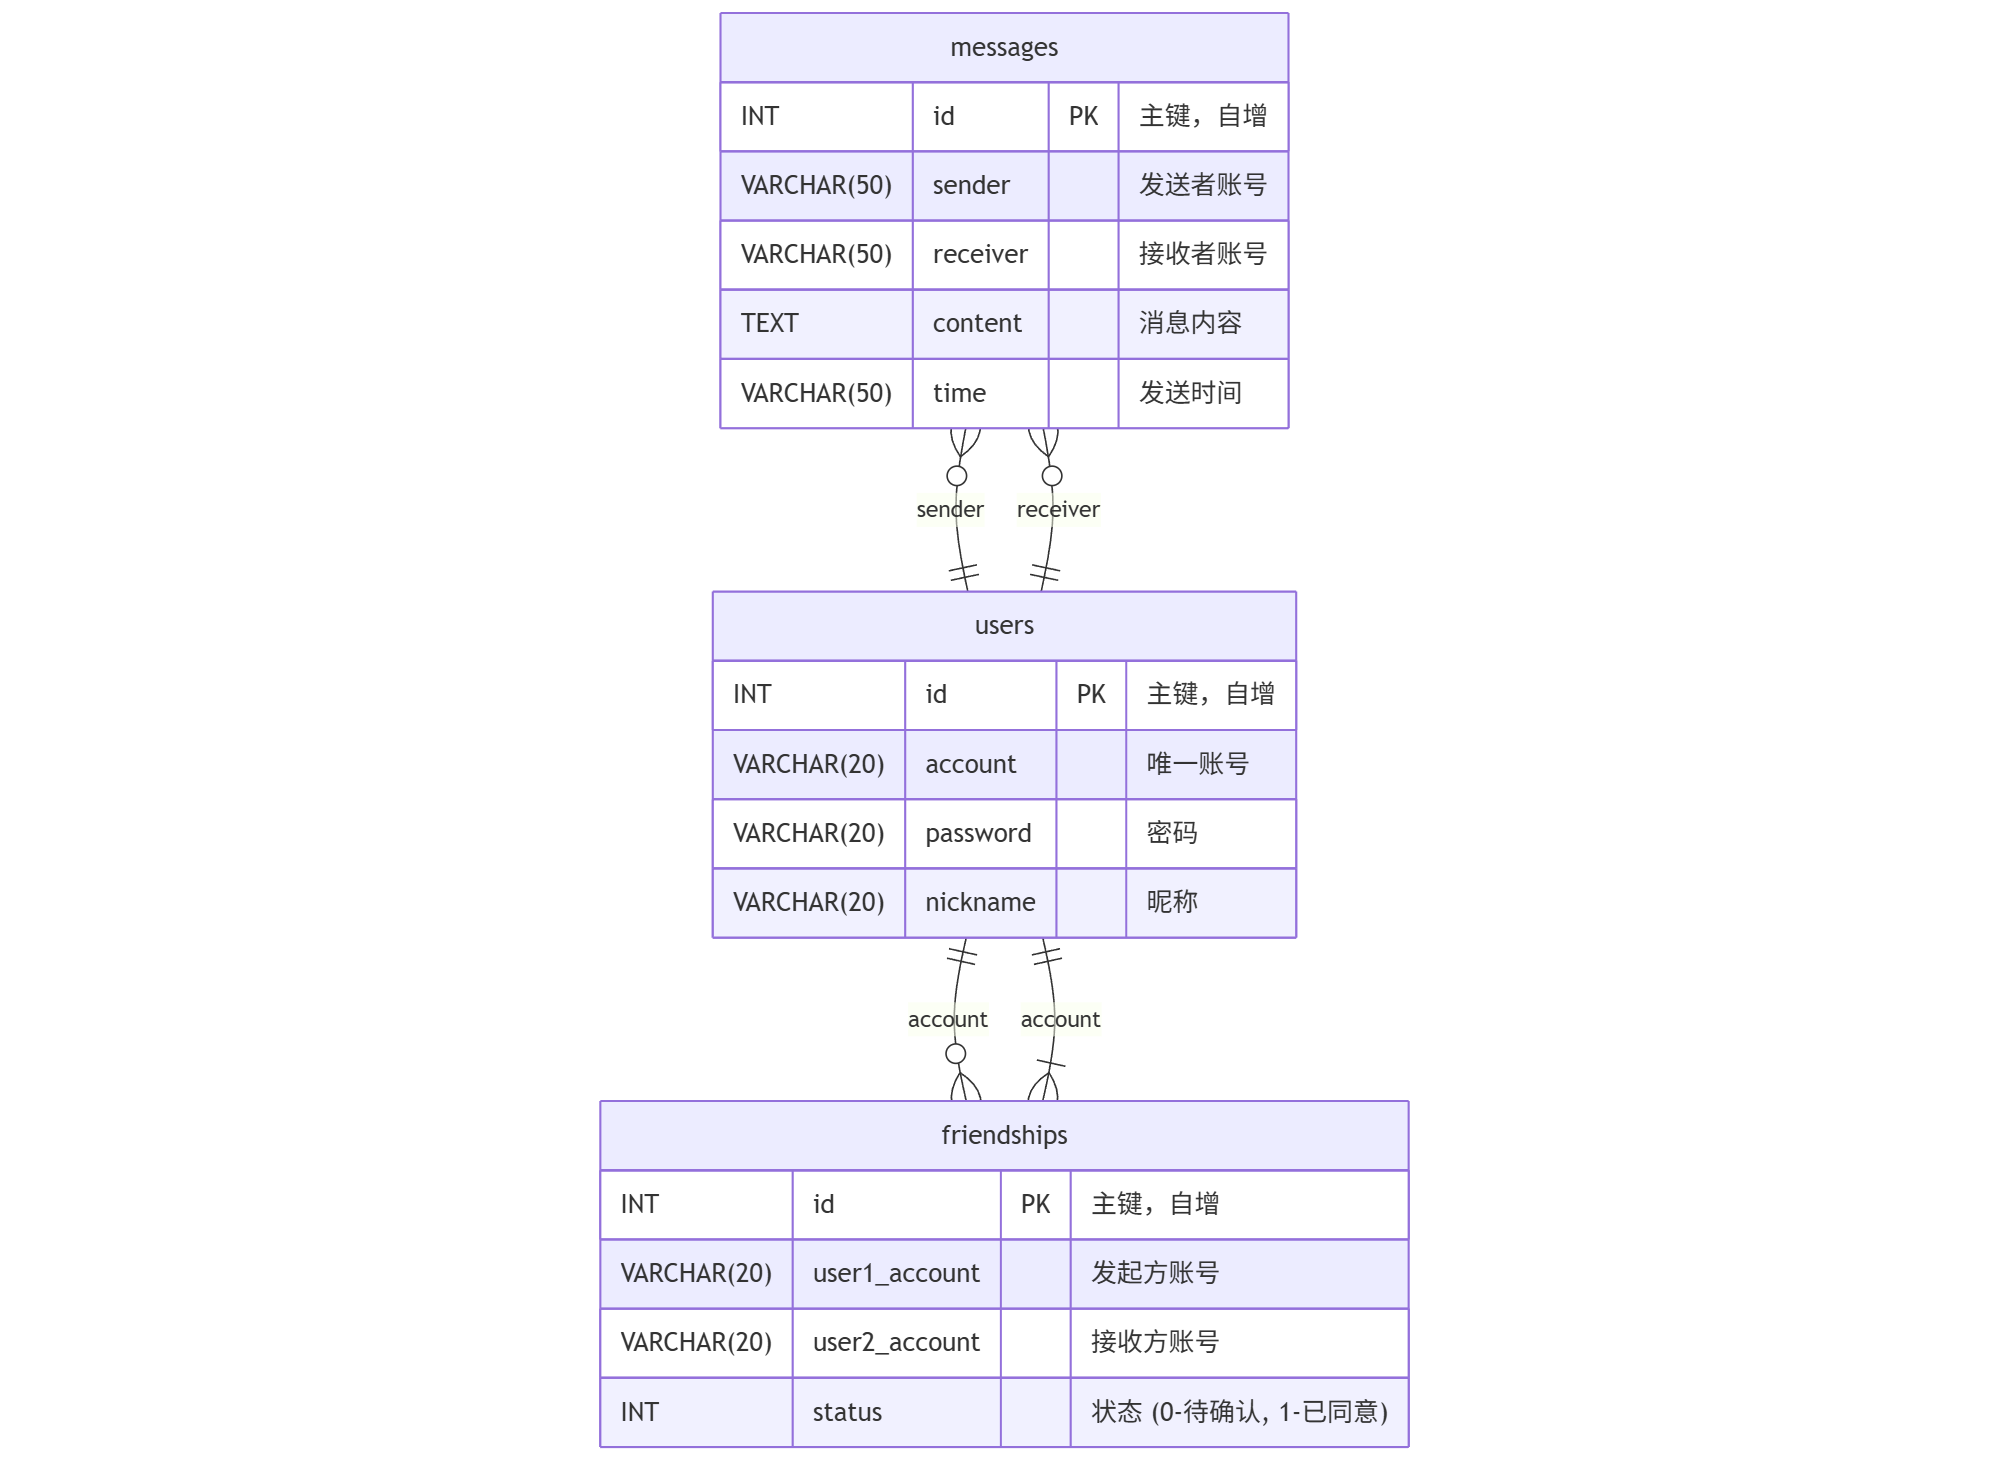
\includegraphics[width=1\textwidth]{sql}
	\caption{数据库设计图}
\end{figure}
\subsubsection{用户表(\texttt{users})}
\begin{table}[h]
	\centering
	\begin{tabular}{|c|c|c|}
		\hline
		字段名 & 数据类型 & 描述 \\
		\hline
		\texttt{account} & \texttt{VARCHAR(20)} & 用户账号(主键) \\
		\texttt{password} & \texttt{VARCHAR(50)} & 密码 \\
		\texttt{nickname} & \texttt{VARCHAR(50)} & 昵称 \\
		\hline
	\end{tabular}
	\caption{用户表(\texttt{users})结构}
	\label{tab:users}
\end{table}

\subsubsection{好友关系表(\texttt{friendships})}
\begin{table}[h]
	\centering
	\begin{tabular}{|c|c|c|}
		\hline
		字段名 & 数据类型 & 描述 \\
		\hline
		\texttt{user1\_account} & \texttt{VARCHAR(20)} & 用户1账号 \\
		\texttt{user2\_account} & \texttt{VARCHAR(20)} & 用户2账号 \\
		\texttt{status} & \texttt{INT} & 好友状态(0:申请中,1:已通过) \\
		\hline
	\end{tabular}
	\caption{好友关系表(\texttt{friendships})结构}
	\label{tab:friendships}
\end{table}

\subsubsection{消息表(\texttt{messages})}
\begin{table}[h]
	\centering
	\begin{tabular}{|c|c|c|}
		\hline
		字段名 & 数据类型 & 描述 \\
		\hline
		\texttt{sender} & \texttt{VARCHAR(20)} & 发送者账号 \\
		\texttt{receiver} & \texttt{VARCHAR(20)} & 接收者账号 \\
		\texttt{content} & \texttt{TEXT} & 消息内容 \\
		\texttt{time} & \texttt{DATETIME} & 发送时间 \\
		\hline
	\end{tabular}
	\caption{消息表(\texttt{messages})结构}
	\label{tab:messages}
\end{table}

\section{类与函数设计}
\begin{figure}
	\centering
	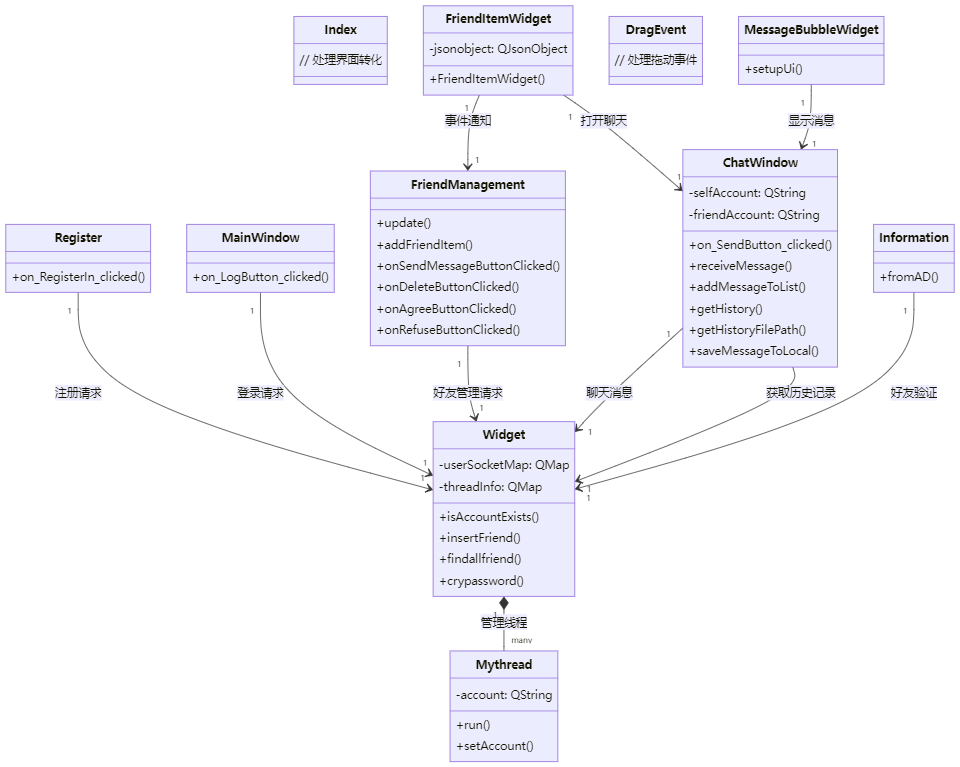
\includegraphics[width=0.5\textwidth]{class}
	\caption{类图}
\end{figure}
\begin{itemize}
	\item \textbf{客户端}
	\begin{itemize}
		\item \texttt{Register}:注册界面类,处理用户注册逻辑。
		\item \texttt{MainWindow}:主窗口类,处理用户登录。
		\item \texttt{ChatWindow}:聊天窗口类,处理消息发送和接收。
		\item \texttt{Index}:主界面类,处理界面转化。
		\item \texttt{FriendManagement}:好友管理界面类,处理好友管理。
		\item \texttt{FriendItemWidget}:好友元素类,用于好友显示。
		\item \texttt{DragEvent}:拖动事件类,处理拖动事件。
		\item \texttt{Information}:信息类,处理用户信息显示与发送好友申请。
		\item \texttt{MessageBubbleWidget}:消息气泡类,处理聊天信息的显示。
	\end{itemize}
	\item \textbf{服务端}
	\begin{itemize}
		\item \texttt{Widget}:服务端主类,处理客户端请求,与数据库交互。
		\item \texttt{Mythread}:线程类,用于实现多线程。
	\end{itemize}
\end{itemize}
\end{document}